\chapter{Análisis del problema}

Con esta investigación también se espera obtemer
un conocimiento más profundo de las dinámicas subyacentes de nuestro algoritmo. 

\section{Diversidad}

Mantener la diversidad es crucial para evitar una convergencia prematura hacía un optimo local. Rosca \cite{Rosca} concluyó que las poblaciones parecían quedar estancadas
en un óptimo local cuando la entropía no cambiaba o decrecía monótonamente en las genereaciones sucesivas. Uno de los objectivos de este trabajo es investigar como la 
división en castas afecta a la diversidad. En programación genética, la diversidad se refiere a diferencias estructurales, como por ejemplo la cantidad de genotipos 
distintos en la población o la singularidad de valores del fitness \cite{genetic}. Hay diferentes medidas para calcularla, entre ellas: diversidad genotípica, 
diversidad fenotípica, entropía, pseudo isomorfismo, distancias de edición, etc. De entre ellas calularemos la \textbf{entropía}, que describe como se distribuye la
población entorno a los diferentes valores del fitness, y la \textbf{distancia de edición}, en la que cada individuo se mide contra el mejor individuo encontrado hasta el 
momento. Se han elegido porque según Burke \cite{diversity} la entropía y la distancia de edición muestran una gran correlación con el aumento y decremento de el valor 
del fitness. Una vez calculadas, se investigará la relación entre el fitness y la  diversidad \cite{diversity}. 

\subsection{Experimentos}

Para realizar estas pruebas usaremos la configuración de la Tabla \ref{tab:diversity_config}, como función a minimizar la función Rastrigin\cite{BBOB}, y la distancia Euclidea.

\begin{table}[]
    \centering
    \begin{tabular}{||c|c||}
        \hline
        \multicolumn{2}{|l|}{\textbf{Fichero Configuración: config\_file\_1.json}} \\ \hline
        Tamaño cromosoma                                & 2               \\ \hline
        Tamaño de la población                          & 100             \\ \hline
        Máximo de generaciones                          & 15              \\ \hline
        Porcentaje Alpha de la población                & 10              \\ \hline
        Porcentaje Beta de la población                 & 20              \\ \hline
        Porcentaje Gamma de la población                & 20              \\ \hline
        Porcentaje Delta de la población                & 20              \\ \hline
        Porcentaje Epsilon de la población              & 30              \\ \hline
        Ratio de mutación                               & 10              \\ \hline
    \end{tabular}
    \caption{Parámetros de configuración para exploración de la diversidad}
    \label{tab:diversity_config}
\end{table}

\begin{figure}[H]
	\centering	
	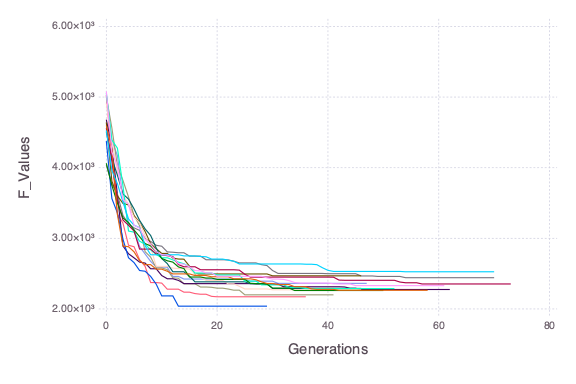
\includegraphics[scale=0.6]{figuras/config_file_1_Rastrigin.png}
	\caption{Primera ejecución}
    \label{fig:primera_ejecucion}
\end{figure}

En la Figura \ref{fig:primera_ejecucion} se ve el resultado de ejecutar el algoritmo 15 veces con la configuración anterior.
Se puede ver como los mejores resultados se obtienen en las primeras generaciones. La mayoría de las ejecuciones muestran como la mejora
del fitness disminuye alrededor de la generación 15-20, y como a partir de la 40 deja de mejorar. Esto puede indicar que cuanto mayor es la generación menor es la 
diversidad. Para apoyar esta idea tenemos las Figuras \ref{fig:best_f_value} y \ref{fig:worst_f_value}. 

La Figura \ref{fig:best_f_value} muestra la diversidad de la ejecución que resulta en un mejor fitness, de la generación 20 a la 30 es donde hay una 
disminución mayor de la entropía lo que provocará el estancamiento en un óptimo local. En la segunda imagen se ve como la entropía va disminuyendo, sin 
embargo tiene picos, lo que provoca que el algoritmo aguante 30 generaciones más que la anterior, aún sin llegar a superar el fitness de la población anterior. En
ambas imágenes se ve como la distancia de edición refleja completamente la tendencia del fitness. Además, entorno a la generación 20 dicha distancia se mantiene
en valores parecidos, resultando en una diversidad más pobre.

\begin{figure}[]
	\centering	
	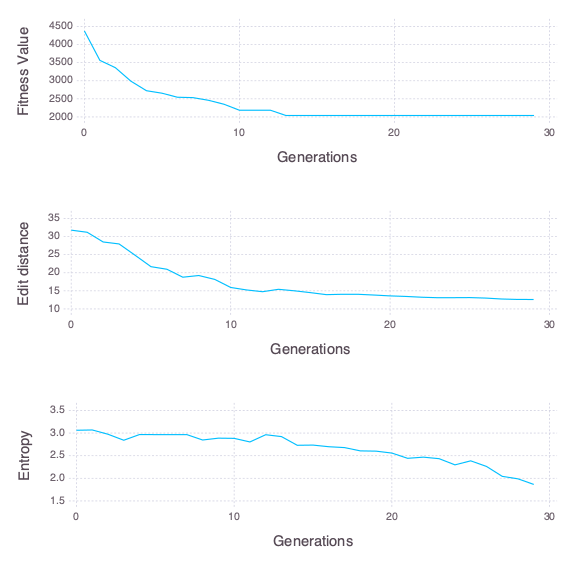
\includegraphics[scale=0.5]{figuras/config_file_1_Rastrigin_best_f_value.png}
	\caption{ Diversidad en la ejecución con mejor resultado de fitness }
    \label{fig:best_f_value}
\end{figure}

\begin{figure}[]
	\centering	
	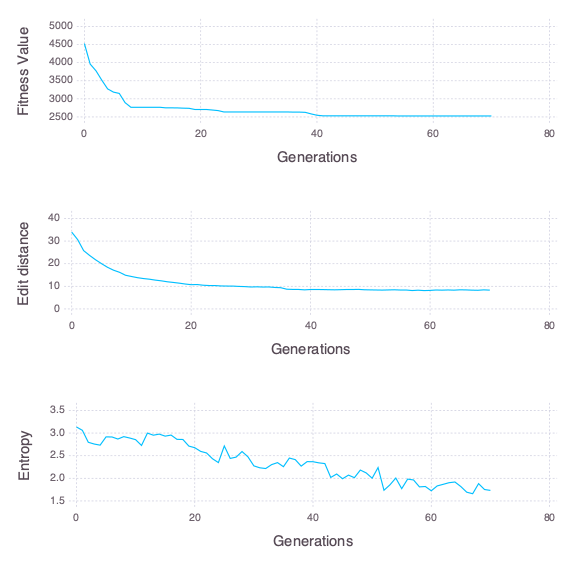
\includegraphics[scale=0.5]{figuras/config_file_1_Rastrigin_worst_f_value.png}
	\caption{ Diversidad en la ejecución con peor resultado de fitness }
    \label{fig:worst_f_value}
\end{figure}

\section{Exploración inicial}

El objetivo de exta exploración escoger los parámetros : dimensión del cromosoma (\textit{DIM}) y tamaño de población. Primero se varia la dimensión
del cromosoma y la población se mantiene fija a 100. Se ejecutará el algoritmo 15 veces por cada dimensión del cromosoma, y se cogerá el que 
tenga mejor resultado para la comparación. Los resultados de esta primera exploración se encuentran en la Tabla \ref{tab:fitness_variation}. 


\begin{table}[]
    \centering
    \begin{tabular}{||c|c|c|c|c||}
        \hline
        \textbf{Fichero Configuración} & \textbf{Generaciones} & \textbf{DIM} & \textbf{Tiempo de ejecución} & \textbf{Mejor fitness} \\ \hline
        Config File 1   & 30    & 2   & 5.1160  & 2039.487   \\ \hline
        Config File 2   & 41    & 3   & 5.4659  & 1989.754   \\ \hline
        Config File 3   & 32    & 5   & 5.1378  & 2068.954   \\ \hline
        Config File 4   & 42    & 10  & 4.9277  & 1971.862   \\ \hline
        Config File 5   & 46    & 20  & 4.7593  & 2059.756   \\ \hline
        Config File 6   & 50    & 40  & 5.9441  & 2123.195   \\ \hline
    \end{tabular}
    \caption{Resultados exploración inicial}
    \label{tab:fitness_variation}
\end{table}


Para un tamaño de población 100 la mejor dimensión es la 4. Sin embargo obsevando la Figura \ref{fig:box_plots} se puede ver que se trata de
un caso atípico, por lo que no podemos concluir con precisión de que sea la mejor configuración. De la figura también se puede extraer que 
los valores de la función objetivo apenas varían si variamos la dimensión del cromosoma, en todos los casos tienen una mediana parecida.

\begin{figure}[]
	\centering	
	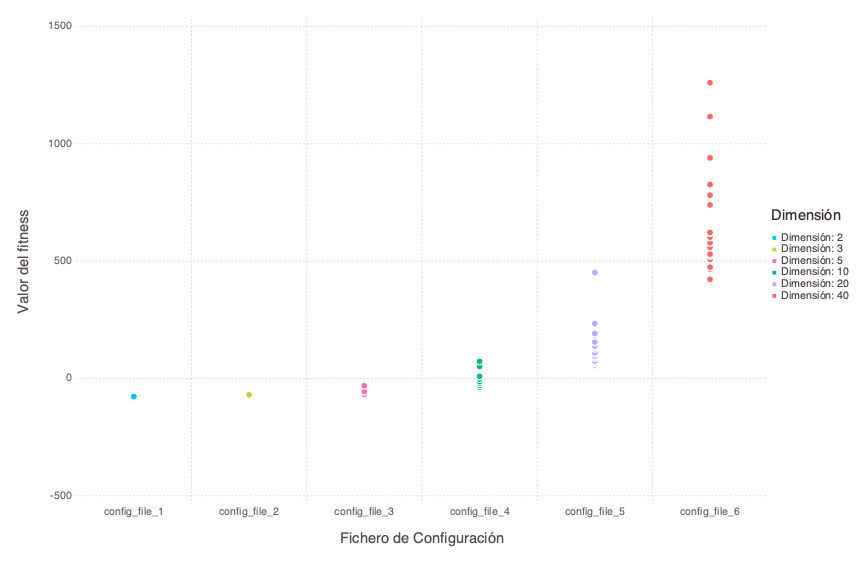
\includegraphics[scale=0.4]{figuras/config_file_1-6_Rastrigin_box_plots.png}
	\caption{ Variación del valor del fitness }
    \label{fig:box_plots}
\end{figure}

Esta exploración no ha dado mucha información. En las siguientes secciones se le dará un enfoque diferente. Primero se buscará un valor de
tamaño de población base, que luego variará proporcionalmente con la dimensión.


\section{Exploración población inicial base}

El objetivo de esta sección es obtener una población inicial base para las próximas exploraciones. Dejaremos fija la dimensión del cromosoma,
será tamaño 2. Se ha escogido esta dimensión porque en la Figura \ref{fig:box_plots} es la que tiene menor mediana.




\begin{table}[]
    \centering
    \begin{tabular}{||c|c|c|c|c||}
        \hline
        \textbf{Fichero Configuración} & \textbf{Generaciones} & \textbf{Tamaño de la población} & \textbf{Mejor fitness} \\ \hline
        Config File 1   & 30    & 5.1160  & 2039.487   \\ \hline
        Config File 7   & 41    & 5.4659  & 1989.754   \\ \hline
        Config File 8   & 32    & 5.1378  & 2068.954   \\ \hline
        Config File 9   & 42    & 4.9277  & 1971.862   \\ \hline
        Config File 10   & 46    & 4.7593  & 2059.756   \\ \hline
    \end{tabular}
    \caption{Resultados exploración inicial}
    \label{tab:base_population}
\end{table}



\section{Análisis de las soluciones}

- en que casos da mejor resultado y por qué, comparar con hipótesis inicial
- Por qué da mejores resultados con una funcion o con otra o con respecto al algoritmo genetico


\subsection{Con Búsqueda Local}

% TODO: hacer la misma tabla para diferentes tamaños de población
\begin{tabular}{||c|c|c|c|c||}
    \hline
    \textbf{Fichero Configuración} & \textbf{Función} & \textbf{DIM} & \textbf{Tiempo de ejecución} & \textbf{Mejor elemento} \\ \hline
    example                                     & example          & 2      & example                      & example                 \\ \hline
                                                &                  & 3             &                              &                         \\ \hline
                                                &                  & 5             &                              &                         \\ \hline
                                                &                  & 10             &                              &                         \\ \hline
                                                &                  & 20             &                              &                         \\ \hline
                                                &                  & 40             &                              &                         \\ \hline

\end{tabular}

